\section{Experiments}
\label{sec:experiment}



\begin{algorithm}[h]
\caption{Practical Score-induced Latent Diffusion (SiLD)}
\label{alg:practical-sild}


% \subsection{Practical Score-induced Latent Diffusion (SiLD)} \label{app:sild}

\begin{algorithmic}[1]

\Require Dataset $\mathcal D$; deterministic encoder
$E_\phi:\mathbb R^d\to\mathbb R^{d_z}$ and decoder $G_\psi$;
latent diffusion network $\epsilon_\theta$;
low-noise and latent time-sampling distributions
$q_{\mathrm{low}}$ and $q_{\mathrm{lat}}$;
latent noise schedule $\{\bar\alpha_t^{\mathrm{lat}}\}$
with $\bar\alpha_T^{\mathrm{lat}}\approx 0$

\Statex \textbf{Stage 1: Low-noise geometric representation learning}

\For{each minibatch $x_0 \sim \mathcal D$}
    \State Sample $t_1 \sim q_{\mathrm{low}}$ and
    $\epsilon \sim \mathcal N(0,I_d)$

    \State
    $x_{t_1} \gets
    \sqrt{\bar\alpha_{t_1}}x_0
    +
    \sqrt{1-\bar\alpha_{t_1}}\epsilon$

    \State
    $\hat{x}_0 \gets G_\psi(E_\phi(x_{t_1}))$

    \State
    $\mathcal L_{\mathrm{stage1}}
    \gets
    \lVert \hat{x}_0-x_0\rVert_2^2$

    \State Update $(\phi,\psi)$ using
    $\mathcal L_{\mathrm{stage1}}$
\EndFor

\State Freeze $E_\phi$ and $G_\psi$

\Statex \textbf{Stage 2: Density learning in the learned coordinates}

\For{each minibatch $x_0 \sim \mathcal D$}
    \State $z_0 \gets E_\phi(x_0)$

    \State Sample $t_2 \sim q_{\mathrm{lat}}$ and
    $\xi \sim \mathcal N(0,I_{d_z})$

    \State
    $z_{t_2}
    \gets
    \sqrt{\bar\alpha_{t_2}^{\mathrm{lat}}}z_0
    +
    \sqrt{1-\bar\alpha_{t_2}^{\mathrm{lat}}}\xi$

    \State
    $\mathcal L_{\mathrm{stage2}}
    \gets
    \lVert
    \epsilon_\theta(z_{t_2},t_2)-\xi
    \rVert_2^2$

    \State Update $\theta$ using $\mathcal L_{\mathrm{stage2}}$
\EndFor

\Statex \textbf{Sampling}

\State Sample $z_T \sim \mathcal N(0,I_{d_z})$
\State Run the standard latent reverse diffusion process to obtain $z_0$
\State \Return $G_\psi(z_0)$

\end{algorithmic}
\end{algorithm}

%A synthetic illustration of two-stage training is presented in the appendix. 
% Algorithm~\ref{alg:practical-sild} shown in Appendix \ref{app:sild} is a theory-inspired practical
% implementation of the two-stage principle. The theoretical guarantees
% above concern the analyzed score-learning procedure. We evaluate practical SiLD on
% image and molecular generation benchmarks. We compare SiLD against LDM~\citep{rombach2022high}, a standard latent diffusion model with a VAE encoder trained with KL regularization. All models share the
% same backbone and training budget to ensure a fair comparison. For
% images, we report Fr\'echet Inception Distance (FID)~
% \citep{heusel2017gans} for generation quality; For molecules, we report validity, uniqueness, novelty
% (fraction of valid generations absent from the training set), internal
% diversity (IntDiv), drug-likeness (QED)~
% \citep{bickerton2012quantifying}, and Fr\'echet ChemNet Distance
% (FCD)~\citep{preuer2018frechet}, alongside reconstruction MSE.

Algorithm~\ref{alg:practical-sild} is a theory-inspired
implementation; the guarantees above concern the analyzed two-stage
procedure. We evaluate practical SiLD against architecture-matched
LDM~\cite{rombach2022high} baselines on image and molecular benchmarks.
For images, we report FID~\cite{heusel2017gans} and reconstruction MSE;
for molecules, validity, uniqueness, novelty, internal diversity (IntDiv),
QED~\cite{bickerton2012quantifying}, and FCD~\cite{preuer2018frechet}.


\begin{figure}[t]
\centering
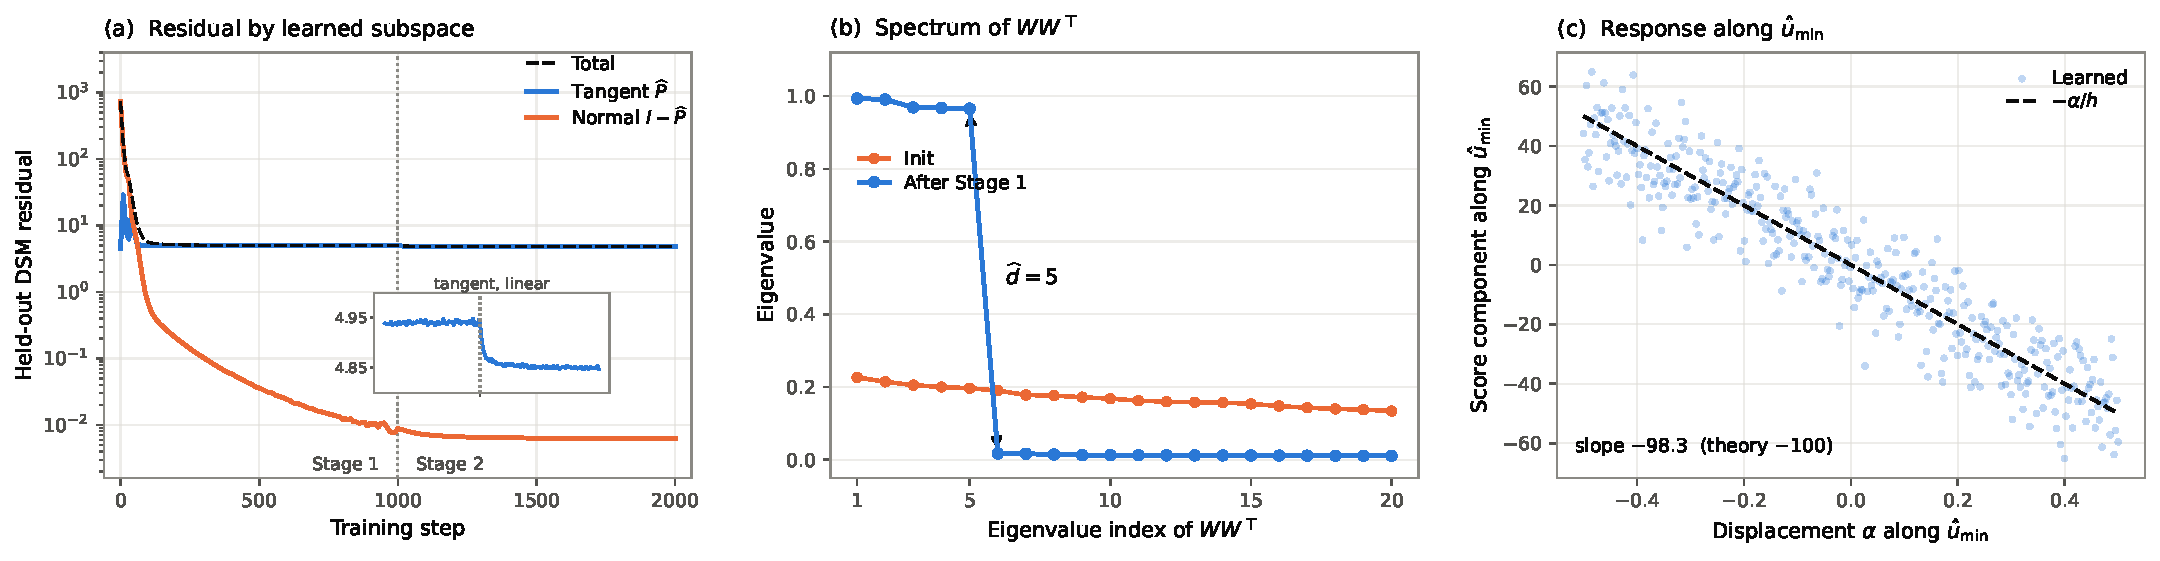
\includegraphics[width=\textwidth]{figures/figure1_no_oracle/figure1_no_oracle_seed42.pdf}
\caption{%
Two-stage training on a synthetic mixture supported on a $k=5$ subspace of
$\mathbb R^{100}$ ($\sigma_t=0.1$, $h_t=\sigma_t^2=10^{-2}$, width $m=200$,
$1000$ steps per stage). All panels use only model- and data-side quantities;
the ground-truth subspace is used to synthesize data, never to compute a
diagnostic. \textbf{(a)} Held-out DSM residual split by the projector
$\widehat P$ onto the model's own top-$\hat d$ eigenvectors. The normal part
falls by five orders of magnitude during Stage~1 and stays flat in Stage~2,
while the tangent part carries essentially all remaining error; the inset
shows the residual Stage-2 gain is confined to the tangent directions.
\textbf{(b)} Spectrum of $WW^\top$ before and after Stage~1: the eigenvalues
separate into $\hat d=5$ near-one directions and a near-zero tail, so the
largest-eigengap estimate recovers the intrinsic dimension without being told
$k$. \textbf{(c)} Learned linear response along the model's own inferred
normal direction $\hat u_{\min}$, with slope $-98.3$ against the predicted
$-1/h_t = -100$.%
}
\label{fig:toy-two-stage}
\end{figure}

\textbf{Synthetic validation.}
Figure~\ref{fig:toy-two-stage} isolates the mechanism behind the two-stage
procedure on a Gaussian mixture supported on a $5$-dimensional subspace of
$\mathbb R^{100}$, using a score network $s_\theta(x)=(\mathrm{ReLU}(xW+b)V^\top
+ xW/h_t)W^\top - x/h_t$ whose linear part is tied to the learned operator
$WW^\top$. Stage~1 trains $W$ with DSM plus an idempotence penalty
$\lVert PP-P\rVert_F^2$, $P=WW^\top$; Stage~2 freezes $W$ and fits only
$(V,b)$. After Stage~1 the operator is numerically a projector (relative
defect $0.043$) of rank $\hat d=5$, matching the true intrinsic dimension,
and the response along the inferred normal directions matches the $-1/h_t$
prediction to within $1.7\%$. The held-out residual splits as
$4.847$ tangent versus $6.2\times10^{-3}$ normal out of a total of
$4.854$: $99.87\%$ of the remaining error lives in the directions Stage~2 is
responsible for, so the two stages learn geometry and density with negligible
interference. As a post-hoc check that no panel depends on,
$\lVert WW^\top - P_{\mathrm{true}}\rVert_F = 0.096$.


%  and mean squared error
% (Recon MSE) and LPIPS~\citep{zhang2018unreasonable} for reconstruction
% quality.


\textbf{Stacked MNIST.}
We evaluate on Stacked MNIST, a 1000-mode benchmark that stacks three random MNIST digits into the R/G/B channels ($d=2352$). SiLD, its $\sigma_{\mathrm{geom}}\!=\!0$ member, and LDM-CNN use matched CNN encoder--decoder backbones and the same latent score architecture, training budget, and Stage-2 interval $t_2\in[0.001,0.999]$. The $\sigma_{\mathrm{geom}}\!=\!0$ member is a clean deterministic autoencoder without KL regularization, whereas SiLD uses additive Stage-1 corruption $x_{\mathrm{noisy}}=x_0+\sigma_{\mathrm{geom}}\epsilon$, with $\sigma_{\mathrm{geom}}=0.005$ and $\epsilon\sim\mathcal N(0,I_d)$. For this experiment, additive corruption replaces the VP form in Algorithm~\ref{alg:practical-sild}; the Stage-1 noise scale is independent of the Stage-2 time interval. All three methods achieve full $1000/1000$ mode coverage (Table~\ref{tab:stacked_mnist}); at matched capacity, SiLD attains $2.0\times$ lower FID ($7.95 \pm 0.26$ vs.\ $16.15 \pm 0.10$, mean$\pm$population std over 3 seeds) and $1.77\times$ lower reconstruction MSE than LDM-CNN. The $\sigma_{\mathrm{geom}}\!=\!0$ member matches SiLD ($8.20 \pm 0.14$; paired per-seed $\Delta\mathrm{FID}=-0.25$, $t=-0.96$, $n=3$): the Stage-1 noise scale is a plateau, and the distinction that carries the effect is whether the Stage-1 map is deterministic at all, not how much noise it sees (Appendix~\ref{app:stage1-noise}).


\begin{table}[t]
\centering
\caption{%
Stacked MNIST (1000-mode benchmark). All three models use matched CNN backbones and the same Stage-2 interval $t_2\in[0.001,0.999]$, with different Stage-1 representation-learning objectives. The second row is the $\sigma_{\mathrm{geom}}\!=\!0$ member of the SiLD family, a clean deterministic autoencoder with no input corruption and no KL term; its difference from SiLD is not significant (paired per-seed $t=-0.96$, $n=3$), so both deterministic arms are marked best. Results are mean$\pm$population std over 3 seeds (42, 43, and 44); all methods achieve full 1000/1000 mode coverage. Appendix~\ref{app:stage1-noise} sweeps the Stage-1 noise scale.%
}
\small
\begin{tabular}{lccc}
\toprule
Stage-1 objective & \#modes / 1000 & Recon MSE $\downarrow$ & FID $\downarrow$ \\
\midrule
Real data           & 1000 & --                                & --                       \\
\midrule
LDM-CNN ($\beta$-VAE AE) & 1000 & $(6.28 \pm 0.05)\!\times\!10^{-3}$ & $16.15 \pm 0.10$ \\
\textbf{SiLD} ($\sigma_{\mathrm{geom}}\!=\!0$; clean AE) & 1000 & $\mathbf{(3.54 \pm 0.04)\!\times\!10^{-3}}$ & $\mathbf{8.20 \pm 0.14}$ \\
\textbf{SiLD (ours)}     &  {1000} & $\mathbf{(3.54 \pm 0.02)\!\times\!10^{-3}}$ & $\mathbf{7.95 \pm 0.26}$ \\
\bottomrule
\end{tabular}
\label{tab:stacked_mnist}
\end{table}





% \begin{table}[t]
% \centering
% \caption{Generation and reconstruction quality on CelebA (64$\times$64).
% All models share identical encoder, decoder, and score network architecture.
% Only the autoencoder training objective differs.}
% \label{tab:celeba}
% \begin{tabular}{llccc}
% \toprule
% \textbf{Method} & \textbf{AE Regularization} & \textbf{FID}$\downarrow$ & 
% \textbf{Recon MSE}$\downarrow$ & \textbf{Eps Loss}$\downarrow$ \\
% \midrule
% LDM (baseline)     & KL divergence        & 43.58 & 0.00265 & \textbf{0.283} \\
% \midrule
% SiLD (ours)          & none                 & 46.22 & 0.00238 & 0.333 \\
% SiLD + MMD (ours)    & MMD ($\alpha{=}0.1$) & 43.56 & 0.00229 & 0.353 \\
% \textbf{SiLD + MMD (ours)} & \textbf{MMD ($\boldsymbol{\alpha{=}1.0}$)} 
%                     & \textbf{42.52} & \textbf{0.00210} & 0.395 \\
% SiLD + MMD (ours)    & MMD ($\alpha{=}5.0$) & 45.59 & 0.00207 & 0.424 \\
% \midrule
% LDM + GAN           & GAN + EMA       & 40.69 & 0.00103 & 0.269 \\
% SiLD + GAN (ours)    & GAN + EMA            & \textbf{39.57} & \textbf{0.00098} & 0.297 \\
% \bottomrule
% \end{tabular}
% \end{table}



% \textbf{CelebA.}
% Table~\ref{tab:celeba} compares SiLD and LDM on CelebA ($64\times64$) at matched architectural capacity, isolating the effect of the Stage-1 objective. At matched regularization strategy, SiLD consistently outperforms LDM: with MMD regularization, SiLD attains $42.52$ FID vs. $43.58$ for KL-regularized LDM; with GAN + EMA, SiLD reaches $39.57$ vs. $40.69$. Reconstruction MSE is lower for SiLD across every setting. The pure, unregularized SiLD variant attains the best reconstruction among KL-free methods ($0.00238$ vs.\ LDM's $0.00265$) but higher FID ($46.22$), reflecting that the latent distribution can contain irregular structures absent any smoothing prior; light auxiliary regularization (MMD or GAN) recovers generation quality while preserving the reconstruction advantage. % At end of CelebA paragraph:
% Similar trends hold on CelebA-HQ ($64\times64\times3$, intrinsic dimension $k_{95} = 223$); see Appendix~\ref{app:celebahq}.

\begin{table*}[t]
\centering
\caption{Unconditional molecule generation on four MoleculeNet benchmarks
(10K samples per method). All methods use SELFIES; validity is checked
with RDKit and FCD against held-out test data. Stage-2 sampling uses the
paired interval $t_2\in[t_0,0.999]$ with $t_0=0.05$; the Stage-1 objective
family, including its $\sigma\!\to\!0$ member and reconstruction error, is
compared at a common $t_2\in[0.001,0.999]$ in
Table~\ref{tab:stage1_family_mol}. Bold indicates the best
generative result for each dataset and metric.}
\label{tab:main_results}
\resizebox{\textwidth}{!}{%
\begin{tabular}{lllcccccc}
\toprule
\textbf{Dataset} & \textbf{Model} & \textbf{Type}
& \textbf{Validity$\uparrow$} & \textbf{Uniqueness$\uparrow$}
& \textbf{Novelty$\uparrow$} & \textbf{Int.\ Div.$\uparrow$}
& \textbf{QED$\uparrow$} & \textbf{FCD$\downarrow$} \\
\midrule
\multirow{7}{*}{\textbf{QM9}}
 & Real data      & ---              & 100.0\% & 96.18\% & 0.0\%   & 0.919 & 0.466 & 5.05 \\
\cmidrule{2-9}
 & CharRNN        & RNN              & \textbf{100.0\%} & 96.32\% & 1.05\%  & 0.917 & 0.465 & 5.13 \\
 & Transformer AR & Transformer      & \textbf{100.0\%} & 96.46\% & 5.26\%  & \textbf{0.920} & 0.465 & 4.98 \\
\cmidrule{2-9}
 & VAE-only       & VAE prior        & \textbf{100.0\%} & 84.43\% & \textbf{88.93\%} & 0.900 & 0.439 & 7.43 \\
 & Latent GAN     & GAN in latent    & \textbf{100.0\%} & 72.63\% & 74.58\% & 0.892 & \textbf{0.474} & 7.80 \\
 & LDM            & Latent diffusion & \textbf{100.0\%} & 96.93\% & 37.6\%  & 0.915 & 0.472 & \textbf{4.28} \\
 & \textbf{SiLD (ours)} & Latent diffusion & \textbf{100.0\%} & \textbf{97.44\%} & 35.9\% & 0.918 & 0.471 & 4.41 \\
\midrule
\multirow{7}{*}{\textbf{HIV}}
 & Real data      & ---              & 100.0\% & 88.93\% & 0.0\%   & 0.898 & 0.513 & 3.24 \\
\cmidrule{2-9}
 & CharRNN        & RNN              & 99.97\% & 88.84\% & 4.39\%  & 0.899 & \textbf{0.514} & 3.24 \\
 & Transformer AR & Transformer      & 99.93\% & 95.16\% & 60.29\% & 0.899 & 0.506 & \textbf{2.91} \\
\cmidrule{2-9}
 & VAE-only       & VAE prior        & \textbf{100.0\%} & 94.18\% & 99.96\% & \textbf{0.912} & 0.388 & 17.66 \\
 & Latent GAN     & GAN in latent    & \textbf{100.0\%} & 95.26\% & 99.99\% & 0.899 & 0.365 & 19.83 \\
 & LDM            & Latent diffusion & \textbf{100.0\%} & 0.96\%  & \textbf{100.0\%} & 0.014 & 0.114 & 60.91 \\
 & \textbf{SiLD (ours)} & Latent diffusion & \textbf{100.0\%} & \textbf{98.74\%} & 99.9\% & 0.904 & 0.430 & 10.43 \\
\midrule
\multirow{7}{*}{\textbf{MUV}}
 & Real data      & ---              & 100.0\% & 95.03\% & 0.0\%   & 0.860 & 0.675 & 4.52 \\
\cmidrule{2-9}
 & CharRNN        & RNN              & \textbf{100.0\%} & 95.12\% & 8.17\%  & 0.862 & \textbf{0.676} & 4.36 \\
 & Transformer AR & Transformer      & \textbf{100.0\%} & 99.33\% & 83.08\% & 0.866 & 0.668 & \textbf{4.06} \\
\cmidrule{2-9}
 & VAE-only       & VAE prior        & \textbf{100.0\%} & 94.98\% & \textbf{100.0\%} & \textbf{0.919} & 0.364 & 33.48 \\
 & Latent GAN     & GAN in latent    & \textbf{100.0\%} & 96.06\% & \textbf{100.0\%} & 0.904 & 0.379 & 34.88 \\
 & LDM            & Latent diffusion & \textbf{100.0\%} & 95.60\% & \textbf{100.0\%} & 0.811 & 0.237 & 41.20 \\
 & \textbf{SiLD (ours)} & Latent diffusion & \textbf{100.0\%} & \textbf{99.42\%} & \textbf{100.0\%} & 0.890 & 0.518 & 19.48 \\
\midrule
\multirow{7}{*}{\textbf{PCBA}}
 & Real data      & ---              & 100.0\% & 98.91\% & 0.0\%   & 0.861 & 0.637 & 9.12 \\
\cmidrule{2-9}
 & CharRNN        & RNN              & \textbf{100.0\%} & 99.53\% & 64.8\%  & 0.864 & \textbf{0.635} & 8.08 \\
 & Transformer AR & Transformer      & \textbf{100.0\%} & \textbf{99.94\%} & 95.12\% & 0.869 & 0.624 & \textbf{7.38} \\
\cmidrule{2-9}
 & VAE-only       & VAE prior        & \textbf{100.0\%} & 91.65\% & 99.74\% & \textbf{0.915} & 0.389 & 28.62 \\
 & Latent GAN     & GAN in latent    & \textbf{100.0\%} & 94.93\% & \textbf{99.82\%} & 0.898 & 0.357 & 30.41 \\
 & LDM            & Latent diffusion & \textbf{100.0\%} & 0.57\%  & 94.7\%  & 0.016 & 0.090 & 77.10 \\
 & \textbf{SiLD (ours)} & Latent diffusion & \textbf{100.0\%} & 98.57\% & 99.8\% & 0.895 & 0.491 & 17.79 \\
\bottomrule
\end{tabular}%
}
\end{table*}

% \begin{table*}[t]
% \centering
% \caption{Unconditional molecule generation results on four MoleculeNet benchmarks.
% All methods evaluated on the same protocol (10K samples, RDKit validity, Frechet ChemNet Distance against held-out test set).
% Our reproductions of prior methods use SELFIES representation for fair comparison.
% Best result per column per dataset in \textbf{bold} (among generative methods, excluding real data).
% $^\ddagger$SELFIES guarantees syntactic validity.
% $^\S$CharRNN/Transformer AR achieve low FCD by partially memorizing training molecules (novelty $<$8\% on QM9).}
% \label{tab:main_results}
% \resizebox{\textwidth}{!}{%
% \begin{tabular}{ll ll cccccc}
% \toprule
% \textbf{Dataset} & \textbf{Model} & \textbf{Type}  & \textbf{Validity$\uparrow$} & \textbf{Uniqueness$\uparrow$} & \textbf{Novelty$\uparrow$} & \textbf{Int.\ Div.$\uparrow$} & \textbf{QED$\uparrow$} & \textbf{FCD$\downarrow$} \\
% \midrule
% %%% ---- QM9 ---- %%%
% \multirow{9}{*}{\textbf{QM9}}
%  & Real data                                     & ---               & 100.0\% & 96.18\% & 0.0\%   & 0.919 & 0.466 & 5.05 \\
% \cmidrule{2-10}
%  & CharRNN$^\S$      & RNN    & \textbf{100.0\%} & 96.32\% & 1.05\%      & 0.917 & 0.465 & 5.13 \\
%  & Transformer AR$^\S$ & Transformer    & \textbf{100.0\%} & 96.46\% & 5.26\%      & \textbf{0.920} & 0.465 & 4.98 \\
% \cmidrule{2-10}
%  & VAE-only            & VAE prior  & \textbf{100.0\%} & 84.43\% & \textbf{88.93\%} & 0.900 & 0.439 & 7.43 \\
%  & Latent GAN        & GAN in latent   & \textbf{100.0\%} & 72.63\% & 74.58\% & 0.892 & \textbf{0.474} & 7.80 \\
%  & LDM     & Latent diffusion  & \textbf{100.0\%} & 96.93\% & 37.6\%  & 0.915 & 0.472 & \textbf{4.28} \\
%  & \textbf{SiLD (ours)}                          & Latent diffusion & \textbf{100.0\%} & \textbf{97.44\%} & 35.9\% & 0.918 & 0.471 & 4.41 \\
% \midrule
% \multirow{9}{*}{\textbf{HIV}}
%  & Real data                                     & ---  & 100.0\% & 88.93\% & 0.0\%   & 0.898 & 0.513 & 3.24 \\
% \cmidrule{2-10}
%  & CharRNN$^\S$    & RNN    & 99.97\% & 88.84\% & 4.39\%  & 0.899 & \textbf{0.514} & 3.24 \\
%  & Transformer AR$^\S$  & Transformer   & 99.93\% & 95.16\% & 60.29\% & 0.899 & 0.506 & \textbf{2.91} \\
% \cmidrule{2-10}
%  & VAE-only     & VAE prior   & \textbf{100.0\%} & 94.18\% & 99.96\% & \textbf{0.912} & 0.388 & 17.66 \\
%  & Latent GAN   & GAN in latent  & \textbf{100.0\%} & 95.26\% & 99.99\% & 0.899 & 0.365 & 19.83 \\
%  & LDM       & Latent diffusion & \textbf{100.0\%} & 0.96\%  & \textbf{100.0\%} & 0.014 & 0.114 & 60.91 \\
%  & \textbf{SiLD (ours)}                          & Latent diffusion & \textbf{100.0\%} & \textbf{98.74\%} & 99.9\% & 0.904 & 0.430 & 10.43 \\
% \midrule
% \multirow{9}{*}{\textbf{MUV}}
%  & Real data                                     & ---              & 100.0\% & 95.03\% & 0.0\%   & 0.860 & 0.675 & 4.52 \\
% \cmidrule{2-10}
%  & CharRNN$^\S$   & RNN    & \textbf{100.0\%} & 95.12\% & 8.17\%  & 0.862 & \textbf{0.676} & 4.36 \\
%  & Transformer AR$^\S$  & Transformer   & \textbf{100.0\%} & 99.33\% & 83.08\% & 0.866 & 0.668 & \textbf{4.06} \\
% \cmidrule{2-10}
%  & VAE-only     & VAE prior   & \textbf{100.0\%} & 94.98\% & \textbf{100.0\%} & \textbf{0.919} & 0.364 & 33.48 \\
%  & Latent GAN    & GAN in latent  & \textbf{100.0\%} & 96.06\% & \textbf{100.0\%} & 0.904 & 0.379 & 34.88 \\
%  & LDM        & Latent diffusion & \textbf{100.0\%} & 95.60\% & \textbf{100.0\%} & 0.811 & 0.237 & 41.20 \\
%  & \textbf{SiLD (ours)}                          & Latent diffusion  & \textbf{100.0\%} & \textbf{99.42\%} & \textbf{100.0\%} & 0.890 & 0.518 & 19.48 \\
% \midrule
% \multirow{9}{*}{\textbf{PCBA}}
%  & Real data      & ---    & 100.0\% & 98.91\% & 0.0\%   & 0.861 & 0.637 & 9.12 \\
% \cmidrule{2-10}
%  & CharRNN$^\S$     & RNN      & \textbf{100.0\%} & 99.53\% & 64.8\%  & 0.864 & \textbf{0.635} & 8.08 \\
%  & Transformer AR$^\S$  & Transformer  & \textbf{100.0\%} & \textbf{99.94\%} & 95.12\% & 0.869 & 0.624 & \textbf{7.38} \\
% \cmidrule{2-10}
%  & VAE-only      & VAE prior     & \textbf{100.0\%} & 91.65\% & 99.74\% & \textbf{0.915} & 0.389 & 28.62 \\
%  & Latent GAN    & GAN in latent    & \textbf{100.0\%} & 94.93\% & 99.82\% & 0.898 & 0.357 & 30.41 \\
%  & LDM          & Latent diffusion  & \textbf{100.0\%} & 0.57\%  & 94.7\%  & 0.016 & 0.090 & 77.10 \\
%  & \textbf{SiLD (ours)}                          & Latent diffusion  & \textbf{100.0\%} & 98.57\% & \textbf{99.8\%} & {0.895} & 0.491 & 17.79 \\
% \bottomrule
% \end{tabular}%
% }
% \end{table*}

\textbf{Molecular generation.}
We evaluate on four MoleculeNet benchmarks (QM9, MUV, HIV, PCBA) using the SELFIES representation~\cite{krenn2020self}, which guarantees syntactic validity by construction and thus isolates \emph{distributional} learning as the object of comparison. SiLD and LDM share identical MLP encoder, decoder, and latent score network ($\sim$13M parameters); only the Stage-1 objective differs. We additionally compare against CharRNN, a 2-layer LSTM at matching scale, and report prior string-based methods on QM9 for external reference. Additional baselines are
CharRNN~\citep{segler2018generating},
Transformer AR~\citep{wang2023cmolgpt,noutahi2024gotta},
VAE-only~\citep{gomez2018automatic}, and
Latent GAN~\citep{prykhodko2019novo}.

% Table~\ref{tab:main_results} reports the results. On QM9 (small molecules), SiLD and LDM both match the reference distribution closely, with SiLD slightly ahead on uniqueness ($97.44\%$ vs.\ $96.93\%$) and IntDiv ($0.918$ vs.\ $0.915$). The comparison separates dramatically on the larger, drug-like datasets (HIV, MUV, PCBA): {LDM undergoes distributional collapse}, with uniqueness dropping to $0.96\%$ on HIV, $95.60\%$ on MUV, and $0.57\%$ on PCBA, and IntDiv collapsing to $0.014$--$0.811$ (versus real-data values of $0.86$--$0.90$). In contrast, SiLD preserves the distribution: uniqueness $98.57\%$--$99.42\%$, IntDiv $0.890$--$0.904$, all within close range of the real training distribution. FCD shows the same pattern --- on PCBA, SiLD achieves $17.79$ versus LDM's $77.10$ (real-data self-reference $9.12$). SiLD, in contrast, achieves near-perfect novelty ($99.9\%$--$100\%$) while preserving distributional structure, directly demonstrating that the Stage-1 objective produces a latent faithful to the data manifold rather than collapsing onto it or memorizing from it.
Table~\ref{tab:main_results} shows mixed results on QM9: SiLD slightly
improves uniqueness and IntDiv over LDM, but has a higher FCD. On HIV,
MUV, and PCBA, SiLD improves uniqueness, IntDiv, and FCD over LDM while
maintaining at least $99.8\%$ novelty. The gap is most pronounced on HIV
and PCBA, where LDM's uniqueness falls below $1\%$; on PCBA, SiLD reduces
FCD from $77.10$ to $17.79$. Transformer AR nevertheless achieves the
lowest FCD on HIV, MUV, and PCBA. The $\sigma\!\to\!0$ member of the SiLD
family matches SiLD on all four datasets and is separated from the
KL-regularized bottleneck by the same margin, so here too the active
ingredient is the determinism of the Stage-1 map rather than its noise scale
(Appendix~\ref{app:stage1-family-mol}). Decomposing the pipeline locates the
KL-regularized failure in Stage~1 rather than in the latent diffusion:
encoding real HIV molecules and decoding them already returns $0.95\%$ unique
outputs, and $99.6\%$ of the raw latent coordinates carry standard deviation
below $10^{-3}$, against none for SiLD (Appendix~\ref{app:collapse}).

% CharRNN, the autoregressive baseline, matches the real-data distribution tightly but mostly by \emph{memorizing}: novelty is $1.05\%$ on QM9, $4.39\%$ on HIV --- it reproduces training molecules rather than generating new ones (except on the large PCBA where novelty reaches $64.8\%$).

% Appendix material for this section lives in figures/exp_append.tex
% (input it after \appendix). It defines app:stage1-noise,
% app:stage1-family-mol, app:stage2-tmin, app:collapse, app:steps,
% app:novelty-tradeoff, app:celeba-boundary, and app:3d.
